\newpage

\section{Testowanie aplikacji}\label{chapter:testing}

W celu weryfikacji poprawności działania aplikacji został przeprowadzony szereg testów manualnych. Zbadano główne funkcje aplikacji: detekcję gwiazd, kalibrację obrazów oraz cały przepływ przetwarzania 
zdjęć głębokiego nieba. Dodatkowo, na końcu połączono wszystkie wykonane zdjęcia obiektu NGC1499 w plik wynikowy wraz z kalibracją w celu weryfikacji poprawności działania aplikacji na 
rzeczywistych danych astronomicznych. Proces wykonania danych testowych oraz opis zestawów został przedstawiony w rodziale \ref{chapter:data_acquisition}.

Detekcja gwiazd została zweryfikowana na podstawie zdjęcia referencyjnego z zestawu danych Zestaw1499\_10. Program przygotowano do wykrycia gwiazd zgodnie z ustalonymi parametrami detektora przedstawionymi
w kodzie źródłowym \ref{lst:register_params}. Następnie, na podstawie wykrytych pozycji gwiazd, zostały naniesione znaczniki na zdjęcie referencyjne przedstawione na rysunku \ref{fig:first_with_stars}. 
Gwiazdy zostały poprawnie wykryte na podstawie naniesionych znaczników. Zauważono, że parametry detektora nie pozwalają na wykrycie mniejszych z gwiazd. Takie dopasowanie parametrów zapewnienia, że
większa ilość wykrytych obiektów będzie pokrywać się pomiędzy kolejnymi zdjęciami w zestawie. Małe gwiazdy z małą jasnościa mają mniejszą szansę na zostanie wykrytymi pomiędzy różnymi zdjęciami
z powodu szumu i zmienności warunków obserwacji.

\begin{figure}[!ht]
    \centering
    \includegraphics[width=0.8\linewidth]{images/first_with_stars.png}
    \caption{Przedstawienie zdjęcia referencyjnego dla zestawu 1499 z oznaczonymi wykrytymi gwiazdami.}
    \label{fig:first_with_stars}
\end{figure}

Kolejnym testem była weryfikacja działania kalibracji obrazów. Największy wpływ na końcową jakość zdjęcia, w kontekście kalibracji, ma redukcja winietowania. Przygotowano dwa zestawy danych na podstawie
zestawu 1499 z całkowitem czasem naświetlania 10 minut: jeden bez wykonanych klatek kalibracyjnych a drugi wraz z pełnym zestawem klatek kalibracyjnych. Nastepnie, dla obu zestawów wykonano pełny przebieg
aplikacji. Aby ocenić redukcję winietowania przez kalibrację, obliczono medianę wartości pikseli w każdej kolumnie i przedstawiono ją na wykresie po normalizacji względem największej mediany. 
Wyniki przedstawiono na rysunku \ref{fig:calibration_chart}. Wartości na osi numeru kolumn zostały pominięte ze względu na brak przydatnych informacji - szerokość obrazu wynosiła 7380 pikseli. 
Dla obu zestawów występują artefakty związane z niedoskonałościami transformacji pomiędzy zdjęciami - w rogach obrazu widoczne są pojedyncze
czarne paski z powodu braku danych. Zestaw bez kalibracji wykazuje wyraźne spadki wartości mediany w kierunku krawędzi obrazu. W skrajnych przypadkach wartość mediany spada do poniżej 50\% wartości
maksymalnej w centrum obrazu. Zestaw z kalibracją wykazuje znacznie mniejsze wahania wartości mediany, co wskazuje na skuteczną redukcję winietowania. Wartości mediany na krawędziach obrazu są powyżej
90\% wartości maksymalnej. Największe wartości mediany występują w prawej części obrazu, spowodowane jest to jednak występowaniem mgławic.

\begin{figure}[!ht]
    \centering
    \includegraphics[width=0.8\linewidth]{images/calibration_chart.png}
    \caption{Porównanie mediany wartości pikseli względem maksymalnej mediany w funkcji numeru kolumny dla obrazów wynikowych z kalibracją i bez kalibracji.}
    \label{fig:calibration_chart}
\end{figure}

\newpage

Przeprowadzono pełny przebieg aplikacji dla zestawu Zestaw1499\_10, wykorzystując metodę średniej do łączenia obrazów. Wynikowy obraz przedstawiono na rysunku \ref{fig:zestaw1499_stacked_average}.
Obraz został zbadany wizualnie w celu wykrycia ewentualnych artefaktów lub błędów w przetwarzaniu. Nie stwierdzono widocznych problemów z jakością obrazu poza artefaktami związanymi 
brakiem danych na niektórych krawędziach. Podczas implementacji programu zdecydowano się na wykorzystanie wartości RGB (0,0,0) w przypadku braku danych na krawędziach obrazu po transformacji.
Alternatywą do tego podejścia jest wykorzystanie odbicia lustrzanego lub powielenie najbliższych pikseli. Jednakże, ze względu na niewielką powierzchnię obrazu dotkniętą tym problemem i 
fałszowaniem rzeczywistego przedstawienia nieba, zdecydowano się na pozostawienie czarnych krawędzi. Krawędzie obrazów astronomicznych są często przycinane w dalszej obróce ze względu na
ograniczoną jakość gwiazd (efekt jest szczególnie widoczny dla obiektywów i niektórych rodzajów tańszych teleskopów). Obraz nie wykazuje również powielania się gwiazd spowodowanego błędami w transformacji
względem obrazu referencyjnego.

\begin{figure}[!ht]
    \centering
    \includegraphics[width=0.8\linewidth]{images/zestaw1499_stacked_average.png}
    \caption{Obraz wynikowy dla zestawu Zestaw1499\_10 uzyskany metodą średniej.}
    \label{fig:zestaw1499_stacked_average}
\end{figure}

Ostatecznie wykonano pełne przejście programu dla zestawu zdjęć przedstawiających obiekt NGC1499. Zestaw zawierał 90 zdjęć - każde o czasie naświetlania 60 sekund. Zestaw ten nie został jednak badany
w dalszej części pracy - służył tylko do weryfikacji poprawności działania aplikacji na rzeczywistych danych astronomicznych. Do łączenia obrazów wykorzystano metodę Kappa-Sigma Clipping. Wynikowy
obraz przedstawiono na rysunku \ref{fig:california_edited}. Obraz został poddany obróce w celu przetestowania danych w ekstremalnych warunkach. Obraz został edytowany przy użyciu programuów
GIMP \cite{gimp} oraz StarNet++ \cite{starnet}. Nawet dla ekstremalnych warunków obróbki zdjęcie wynikowe nie wykazuje widocznych błędów w przetwarzaniu. Gwiazdy nie powielają się, a jednolite tło
wskazuje na wysoki stosunek sygnału do szumu.  Widoczne są również szczegóły struktury NGC1499 i mgławic otaczających gwiazdę Atik.

\begin{figure}[!ht]
    \centering
    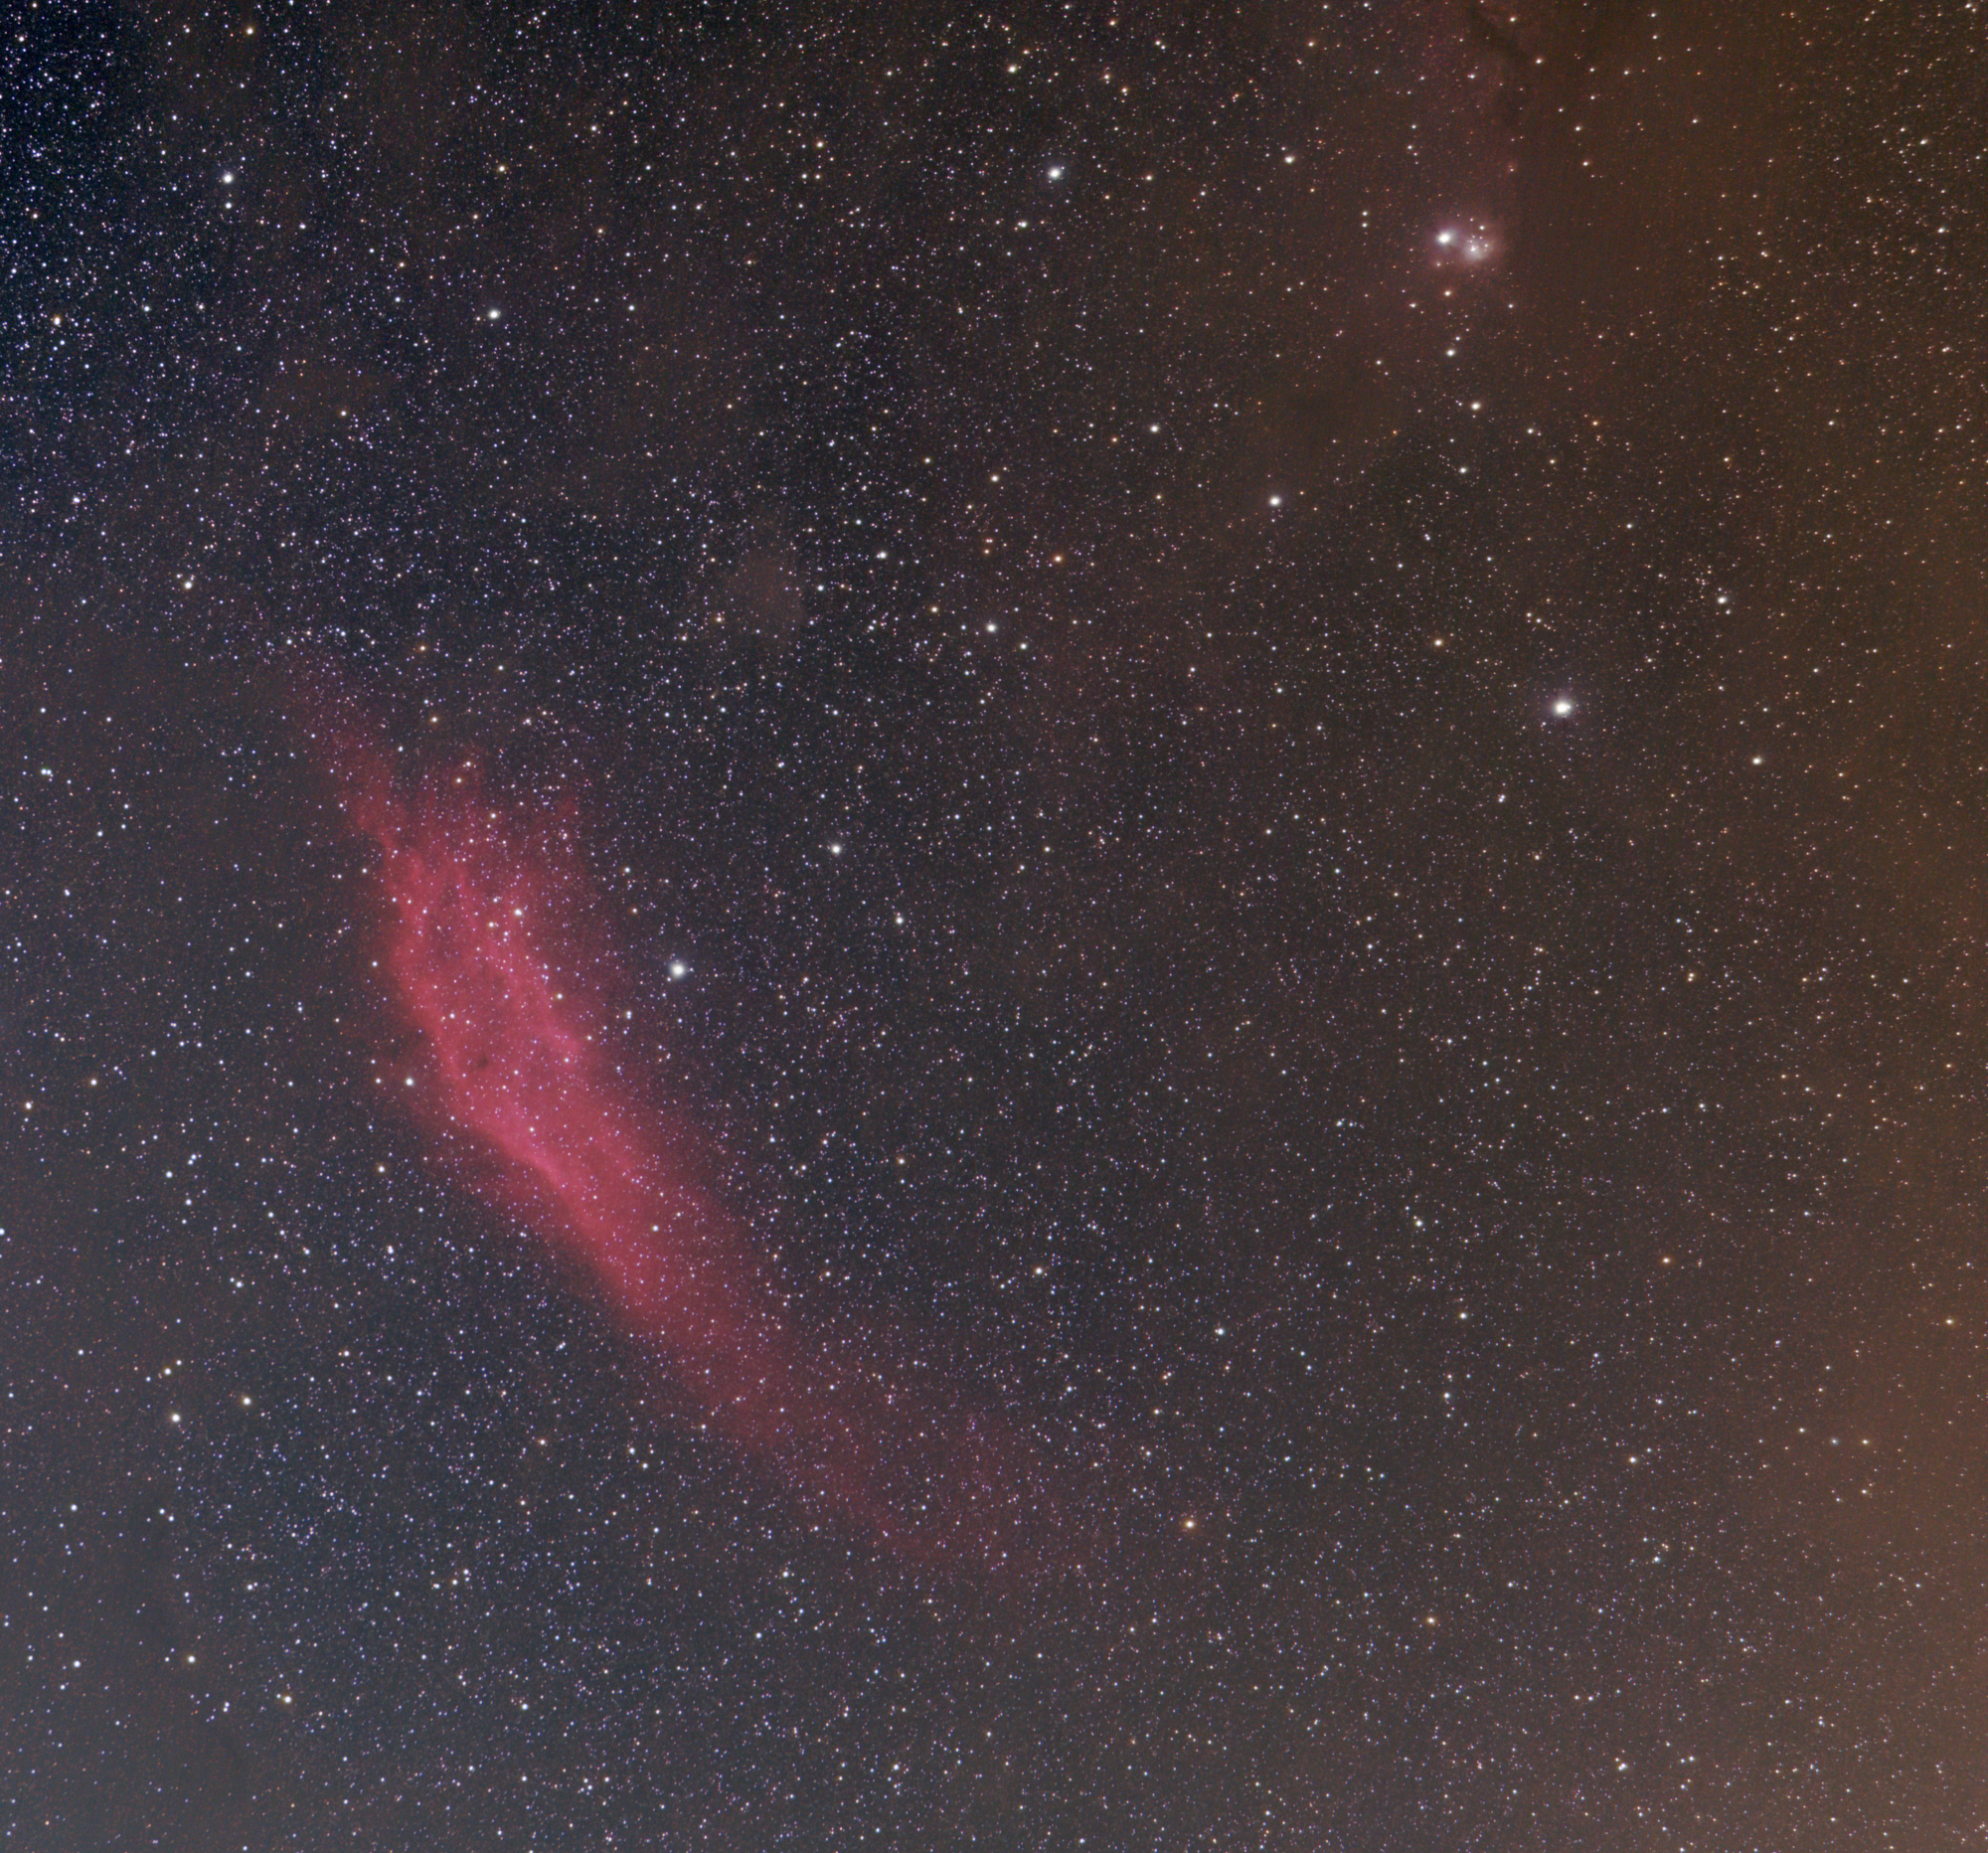
\includegraphics[width=0.6\linewidth]{images/california_edited.png}
    \caption{Edytowany obraz wynikowy obiektu NGC1499 uzyskany metodą Kappa-Sigma Clipping.}
    \label{fig:california_edited}
\end{figure}

